%%%%%%%%%%%%%%%%%%%%%%%%%%%%%%%%%%%%%%%%%%%%%%%%%%%%%%%%%%%%%%%%%%%%%%%%%%%%%%
%arxiv
\documentclass[a4paper,11pt]{article}
% \pdfoutput=1
\usepackage{jcappub}

%%%%%%%%%%%%%%%%%%%%%%%%%%%%%%%%%%%%%%%%%%%%%%%%%%%%%%%%%%%%%%%%%%%%%%%%%%%%%%

\newcommand{\apjs}{ApJ Supplement}
\newcommand{\apj}{ApJ}
\newcommand{\aap}{AAP}
\newcommand{\mnras}{MNRAS}
\newcommand{\prd}{PRD}
\newcommand{\gadget}{{\small GADGET}}
\newcommand{\mpgadget}{{\small MP-GADGET}}

\newcommand{\km}{k_{max}}

\newcommand{\vect}[1]
  {\mbox{\boldmath ${#1}$}}
\newcommand{\matr}[1]
  {\mbox{\bf \sf{#1}}}
\newcommand{\eq}[1]
  {Eq.~(\ref{equation:#1})}
\newcommand{\eqs}[1]
  {Eqs~(\ref{equation:#1})}
\newcommand{\sect}[1]
  {section~\ref{section:#1}}
\newcommand{\sects}[1]
  {sections~\ref{section:#1}}
\newcommand{\tabl}[1]
  {{\mbox Table~\ref{table:#1}}}
\newcommand{\tabls}[1]
  {{\mbox Tables~\ref{table:#1}}}
\newcommand{\fig}[1]
  {Fig.~\ref{Figure:#1}}
\newcommand{\figs}[1]
  {Figs.~\ref{Figure:#1}}
\newcommand{\sourcesection}[1]{\noindent {\em{#1}} ---}

\def\jcap{JCAP}        % Journal of Cosmology and Astro-Particle Physics

\newcommand{\Lya}{Lyman-$\alpha$}
\newcommand{\Msun}{\, h^{-1} M_\odot}
\newcommand{\Zsun}{Z_\odot}
\newcommand{\NHunit}{cm$^{-2}$}
\newcommand{\sLLS}{\sigma_\mathrm{LLS}}
\newcommand{\Mpc}{\,\mathrm{Mpc}}
\newcommand{\Mpch}{\, h^{-1} \mathrm{Mpc}}
\newcommand{\kpch}{\, h^{-1}\mathrm{kpc}}
\newcommand{\hMpc}{\, h \mathrm{Mpc}^{-1}}
\newcommand{\kms}{km~s$^{-1}$}
\newcommand{\NHI}{N_\mathrm{HI}}

\newcommand{\spb}[1]{\textcolor{red}{[\bf SPB: #1]} }
\newcommand{\AFR}[1]{\textcolor{blue}{[\bf AFR: #1]} }

\newcommand{\edit}[1]{#1}

%opening
\title{Lagrangian Glasses for N-body Simulations of Baryons and Dark Matter}

\author[a,1]{Simeon Bird,\note{Corresponding author}}
\author[b]{Yu Feng}
\author[c]{Chris Pederson}
\author[c]{Andreu Font-Ribera}
\affiliation[a]{Department of Physics \& Astronomy, University of California Riverside,\\ Riverside, CA 92521, USA}
\affiliation[b]{Department of Physics, University of California Berkeley, \\Berkeley, CA 94720, USA}
\affiliation[c]{Department of Physics \& Astronomy, University College London,\\Gower Street, London WC1E 6BT, UK}

\emailAdd{sbird@ucr.edu}
\emailAdd{yfeng1@berkeley.edu}
\emailAdd{christian.pedersen.17@ucl.ac.uk}
\emailAdd{a.font@ucl.ac.uk}

\abstract{
XXXX
}

\begin{document}

\maketitle

\section{Introduction}

Cosmological N-body simulations are a well-established technique for understanding non-linear structure formation. Most simulations considered the total growth of structure in the Universe. These evolve a single fluid, corresponding to a combination of cold dark matter (CDM) and baryons, under gravity, under the approximation that these two components trace each other. However, at early times the baryons couple to radiation and thus have their clustering erased on scales less than the comoving horizon scale at recombination. Furthermore, the well-known baryon acoustic oscillation peak is embedded in the baryonic power spectrum but not in the CDM power spectrum. As the Universe evolves, the process of structure formation gradually erases the difference between baryons and CDM, and at $z=0$ they differ by less than $1\%$. Nevertheless, at higher redshift they differ substantially, by up to $8\%$ at $z=10$ and $3\%$ at $z=2$. These differences may be relevant when interpreting, for example, upcoming observations of the \Lya~forest or future galaxy surveys \cite{Schneider:2016}.

Many simulations including baryons (and modeling their hydrodynamics) include them by initializing both CDM and baryons using the total matter spectrum \cite[e.g.][]{Emberson:2018}. A minority interested in high redshift structure growth initialize CDM and baryons using the transfer functions for their respective species. In this case accurate evolution requires also using separate velocity transfer functions for the CDM and baryons. To avoid infinite forces, baryonic and CDM particles are initially offset by half the mean inter-particle spacing.

There is, however, a well-known problem with such simulations \cite{OLeary:2012, Angulo:2013}. Simulations generally wish to achieve equal mass resolution in baryons and CDM. As $\Omega_\mathrm{b} < \Omega_\mathrm{CDM}$, this implies that the mass of baryonic particles differs from the mass of CDM particles.
\AFR{I find it confusing to say "equal mass resolution" when each species has different particle mass. 
I guess this is simulation jargon, but I'd try to find an alternative way to explain it.}
 These unequal masses can induce unphysical coupling of the lower mass (baryonic) particles to the higher mass (CDM) particles \cite{OLeary:2012}, in extreme cases binding the lighter particles to orbiting the heavier ones. A simple analytic derivation of this effect is shown in Appendix B of Ref.~\cite{OLeary:2012}. Furthermore, linear theory makes a prediction for  as a function of redshift. Ref.~\cite{Angulo:2013} showed that the ratio between the baryon power spectrum, $P_b(k)$, and the CDM power spectrum $P_\mathrm{CDM}(k)$, in Gadget-3 \cite{Springel:2005} simulations does not by default agree with the predictions of linear theory, due to this spurious inter-particle coupling.\footnote{\cite{Angulo:2013} have more power in the baryon component than linear theory predicts. For a similar simulation, we find less power than predicted by linear theory. It is unclear why this discrepancy occurs, but it seems likely to be due to differences in the initial velocity distribution or the exact setup of the initial particle grid.} The practical impact of this effect is fortunately reduced because the coupling conserves total momentum, and thus shows the correct evolution of the total matter spectrum.

Refs~\cite{OLeary:2012, Angulo:2013} showed that spurious couplings can be ameliorated by increasing the gravitational softening length of the particles at high redshift. This is done adaptively, setting the baryonic softening length equal to the SPH smoothing length of the baryonic particles. This effectively disables the short range gravitational force at high redshift, when the Universe is homogeneous and thus SPH smoothing lengths are of order the mean inter-particle spacing. We emphasize that on cosmological scales this procedure cannot be justified on the basis of hydrodynamics. The coupling effect is purely gravitational, and persists even if, as in the simulations of Ref.~\cite{Angulo:2013} and the ones presented here, hydrodynamical pressure forces are disabled. Adaptive softening is thus simply an easy way of increasing the softening only at the high redshifts where particle coupling is most acute. Since the small-scale gravitational force is disabled at high redshift, adaptive softening strongly suppresses the small-scale clustering of the baryons in low density regions outside galaxies. This makes it unsuitable for some applications, in particular simulations of the \Lya~forest. Nevertheless, adaptive softening has widely used in recent simulations \cite[e.g][]{Paco:2018}.\footnote{Ref.~\cite{Valkenburg:2017} instead achieved the same effect by setting the cutoff distance for the small-scale force to a small fraction of the PM grid size.}

An alternative resolution to this problem was proposed by Ref.~\cite{Yoshida:2003}. They showed that the desired relative power between baryons and cold dark matter could be achieved by initializing the particles using two independent Lagrangian glasses, rather than the more standard offset grids. The effect of particle couplings propagates to large scales due to the regular grid structure of the simulation, which means that each low-mass (baryonic) particle is equally perturbed by the local effect of the nearest high mass (cold dark matter) particles. A local perturbation is thus replicated across the box and shows up as a large scale offset from the desired growth. Many of our results are implicit in the results of Ref.~\cite{Yoshida:2003}. However, they did not consider large scales and thus did not include the effect of species and scale dependent velocity transfer functions as we do here.
We show that initializing the baryons using a Lagrangian glass rather than a grid offset from the CDM allows a simulation to reproduce the ratio between CDM and baryons predicted by linear theory. The noise inherent in a glass distribution is reduced by using a glass only for the baryons, not for the CDM. To further prevent chance juxtapositions of CDM and baryon particles we perform a single reverse-gravity timestep on the combined particle distribution, following Ref.~\cite{Yoshida:2003}.

We also show that an alternative technique to reproducing the baryon-CDM offset without deviating from a regular grid nor altering the force law is to over-sample the CDM relative to baryons by a factor of $\Omega_\mathrm{CDM}/\Omega_\mathrm{b}$. This means that each particle species has roughly the same mass and thus the inaccuracies resulting from differing mass particles are removed.

Other possibilities for the initial particle distribution have also been proposed. Ref.~\cite{Hansen:2007} used a quaquaversal tiling of three dimensional space, which we do not consider as it restricts the total number of particles to a power of two. Ref.~\cite{Liao:2018} used a capacity constrained Voronoi tessellation, which preserves most of the good properties og a Lagrangian glass. We do not use it here only because it is not obvious how to generalize it to two fluids.

%I feel strongly that Angulo & Hahn simply wrote a wrong paper - our results agree much better with Yoshida 2003 than them.
%We have never been able to reproduce their results and when we use a glass file we get the right answer.
%They I think probably used the wrong velocity transfer functions.

\section{Methods}

In this Section we describe our methods for initializing cosmological simulations, as well as the simulations we run.

The basic algorithm of our preferred setup is similar to that presented in Ref~\cite{Yoshida:2003} and is as follows:
\begin{enumerate}
 \item Produce a homogeneous distribution of CDM particles arranged in a regular grid.
 \item Produce a homogeneous distribution of gas particles by generating a Lagrangian glass.
 \item Evolve the mixed distribution of both types of particles using a reversed gravitational force, as when generating a Lagrangian glass. This avoids random close juxtapositions of CDM and baryon particles.
 \item Set the velocity of the baryon and CDM particles using the species specific velocity transfer functions, avoiding the Zel'dovich approximation.
  \item Displace the baryon and CDM particles according to their species specific displacement transfer functions.
\end{enumerate}

We do not use second-order Lagrangian perturbation theory \cite{Scoccimarro:1998}, despite its reduced transients as, to our knowledge, the full species specific velocity and displacement second order transfer functions, including baryon-CDM cross-terms, do not exist in the literature. We defer this to future work.

\subsection{Grid and Glass Particle Distribution Generation}
\label{sec:glass}

We generate glass particle distributions following \cite{White:1994} by evolving a gravitationally interacting N-particle system with the sign of gravity reversed, so that each particle feels repulsive forces from each other particle. We have implemented this  gravitational force evolution directly into our initial conditions code. It uses the same particle-mesh algorithm as in MP-Gadget with a particle mesh grid twice as fine as the mean inter-particle spacing. No short-range tree force is needed as the particle distribution is, by design, extremely homogeneous. The initial particle distribution is a regular grid with the positions of each particle randomized over three mean inter-particle spacings. A symplectic leap-frog is run with a kick-drift-force-kick arrangement for fourteen timesteps. The velocity kick includes a damping term proportional to the velocity to avoid particle positions oscillating around the minimum. \spb{Yu: can you explain the specific choice of damping term more?} The velocity produced by the glass evolution is zeroed after the glass generation is complete. The reverse gravity evolution is done for $14$ timesteps. Every particle is active during every timestep.

This procedure can be applied separately to both CDM and baryons, generating two uniform homogeneous gas distributions.
Although the distribution of each individual particle species is homogeneous, there is no guarantee that this property also applies to
the total particle distribution. The original benefit of a glass, low residual force between all particles, does not hold for two combined glasses \cite{Yoshida:2003} as particles of one species may occasionally, by chance, be initialized extremely close to a particle of a different species. This causes two types of problems: the first is that close pairs of particles causes the computation of the tree force to be computationally expensive as the tree is very deep. The second is that artificial structure will be seeded at some level in the small regions around the close particles, causing a deviation from linear theory on small scales.

We investigated generating a single coherent glass file containing both species of particle. In this glass file both particle species are placed at random and then evolved with reversed gravity to a single, coherent, homogeneous distribution. However, this contained no mechanism for keeping the distribution of each species homogeneous, and thus produced a density map which had overdensities of baryons exactly compensated by overdensities of cold dark matter. This in turn led to very noisy power spectrum estimation as not all modes were fully sampled. Furthermore, in a realistic hydrodynamical simulation it would have caused, for example, dark matter halos containing no baryons to form, leading to strange numerical artifacts.

Ref.~\cite{Yoshida:2003} proposed a resolution to reduce chance alignments of two particle species. After generating two separate homogeneous glass files, they ran a single reversed-gravity timestep on the combined particle distribution. This ensures that particles which are exceptionally close by chance are disrupted, but does not disrupt the overall glass distribution of the simulation. We extended this work and considered the effect of running $14$ reversed gravity timesteps on the combined particle distribution, so that the overall particle distribution is homogeneous. \spb{Yu, why 14?}

Our use of a glass distribution is designed solely to remove the regular coupling between baryons and cold dark matter inherent in an offset particle grid and thus reproduce correctly the relative evolution of the two species. For this reason we generate a glass distribution for baryonic particles, and a regular grid for cold dark matter. The glass noise is still present, but at a reduced level because baryons are only $\sim 1/6$ of the total matter. For realistic simulations the noise would be further damped by pressure forces, although these are not included in the simple toy examples performed here.

We compared the results of this procedure to starting from glasses for both CDM and baryons and found the differences between them to be minor. However, in our tests evolving a coherent glass starting from a regular grid for the CDM was marginally easier to set up and led to marginally better agreement with linear theory, so we chose to use it throughout.

We also considered using $4$ timesteps rather than $14$ timesteps for the reversed gravity evolution of the combined CDM grid and baryonic glass. We found minimal difference in the final power spectra, but the extra timesteps did moderately reduce the number of close particle pairs in the simulation with some improvements in computational time, hence we chose to use $14$ timesteps for the combined particle distribution.

%As is well-known \spb{(CITATION?)} the use of a Lagrangian glass causes noise in the particle power spectrum proportional to $k^4$ on scales approaching that of the mean inter-particle spacing\footnote{A regular particle grid instead causes a strong peak in the power spectrum at harmonics of particle grid.}.
%We are satisfied with the properties of a regular grid for initializing cold dark matter density fields, and consider the systematics at the particle grid scale an acceptable trade-off for the reduction in noise on larger scales.

\subsection{Initialization of Particle Velocities and Displacements}

Key to reproducing linear theory is the correct initialization of particle velocities and displacements. Since there are several approximations current in the literature, and the velocity transfer functions in particular are not trivial, we here review the linear results. We do not use the common Zel'dovich approximation, which is:
\begin{equation}
 v = a H(a) \frac{d \ln D_1(a)}{d \ln a} x
\end{equation}
where $x$ is the particle displacement and $D_1(a)$ is the growing mode total matter linear growth factor\footnote{Sometimes this is further approximated as $\Omega_M^{3/5}$, which is indefensible today.}. The growth function for individual species is not the total growth function, so this introduces an inaccuracy in the relative velocities of the baryons and CDM.

Instead we initialize both displacements and velocities directly using the transfer functions from the linear Boltzmann code CLASS \cite{CLASS}, corresponding to the solutions of the equations of linear cosmological perturbation theory in synchronous gauge. We apply a species-independent boost to the velocities, as the CLASS transfer functions are printed in a frame comoving with the cold dark matter. Following the notation of Ref.~\cite{Ma:1995}, we set:
\begin{align}
 v_\mathrm{CDM} = \dot{\delta}_\mathrm{CDM}  &= - \frac{\dot{h}}{2} \\
 v_\mathrm{b} = \dot{\delta}_\mathrm{b}  &= - \theta_\mathrm{b} - \frac{\dot{h}}{2}
\end{align}
where $\dot{h}$ and $\theta_\mathrm{b}$ are set using the relevant columns in the CLASS transfer functions.
Particle displacements are set using the columns for $\delta_\mathrm{CDM, b}$. Note that each of these quantities is fully scale-dependent, so that the scale-dependence of the velocity perturbations is automatically included without having to numerically differentiate the growth factor. The appropriate unit conversions are performed to convert from CLASS to Gadget units\footnote{See: \protect\url{https://github.com/MP-Gadget/MP-Gadget/blob/FirstDOI/libgenic/power.c\#L204}.}.

\subsection{Example Simulations}

We perform toy test simulations with $2\times 256^3$ particles and box sizes of $300$ Mpc/h (comoving). Our initial conditions are generated at $z=99$ and we compare to linear theory power spectra and transfer functions generated using CLASS \cite{CLASS}. We assume a periodic box and a standard $\Lambda$CDM cosmology with $\Omega_\mathrm{M} = 0.3$, $h = 0.67$, $n_s = 0.97$. We have set $\Omega_\mathrm{b} = 0.05$ so that $\Omega_{\mathrm{CDM}}/ \Omega_\mathrm{b} = 5$.
To ensure that structure grows linearly even at low redshifts we artificially suppress the initial power spectrum by a factor of $100$, setting $A_s = 2.14\times 10^{-11}$, and thus $\sigma_8 = 8\times 10^{-3}$.
\AFR{I believe you mean  $\sigma_8 = 8\times 10^{-2}$. 100 times less power, 10 times smaller rms.}

To confirm that our results continue to hold outside of our toy examples we also performed a larger simulation with a box of $1$ Gpc/h (a scale large enough that the baryon and CDM transfer functions are approximately equal on scales of the box) and $768^3$ particles.

Our simulations were performed with the scalable N-body code MP-Gadget \cite{yu_feng_2018_1451799} using the built-in initial conditions generator MP-GenIC. MP-Gadget is descended from P-Gadget3 but has been heavily modified for scalability. Hydrodynamics, pressure forces, cooling and star formation are disabled; despite including particles initialized with a baryonic transfer function, our simulations are purely gravitational.

\begin{table}
\begin{center}
\begin{tabular}{|l|c|c|c|l|}
\hline
Name & Box & $N_\mathrm{CDM}^{1/3}$ & $N_\mathrm{baryon}^{1/3}$ & Comments  \\
\hline
\texttt{TWOGRID}    &   $300$ & $256$ & $256$ & Two offset particle grids. \\
\texttt{ADAPTIVE}    &   $300$ & $256$ & $256$ & As TWOGRID but adaptive gas softenings. \\
\texttt{UNDERSAMP}  &   $300$ & $256$ & $150$ & Two offset particle grids, same particle masses. \\
\texttt{HALFGLASS}  &   $300$ & $256$ & $256$ & Baryons on a glass, CDM on a grid, see text. \\
\texttt{BIGGLASS}  &   $1000$ & $768$ & $768$ & As HALFGLASS. \\
\hline
\end{tabular}
\end{center}
\caption{Table of simulations. Box size is in comoving Mpc/h. $\sigma_8 = 0.008$ throughout.}
\label{tab:simulations}
\end{table}

\section{Results}

\begin{figure}
  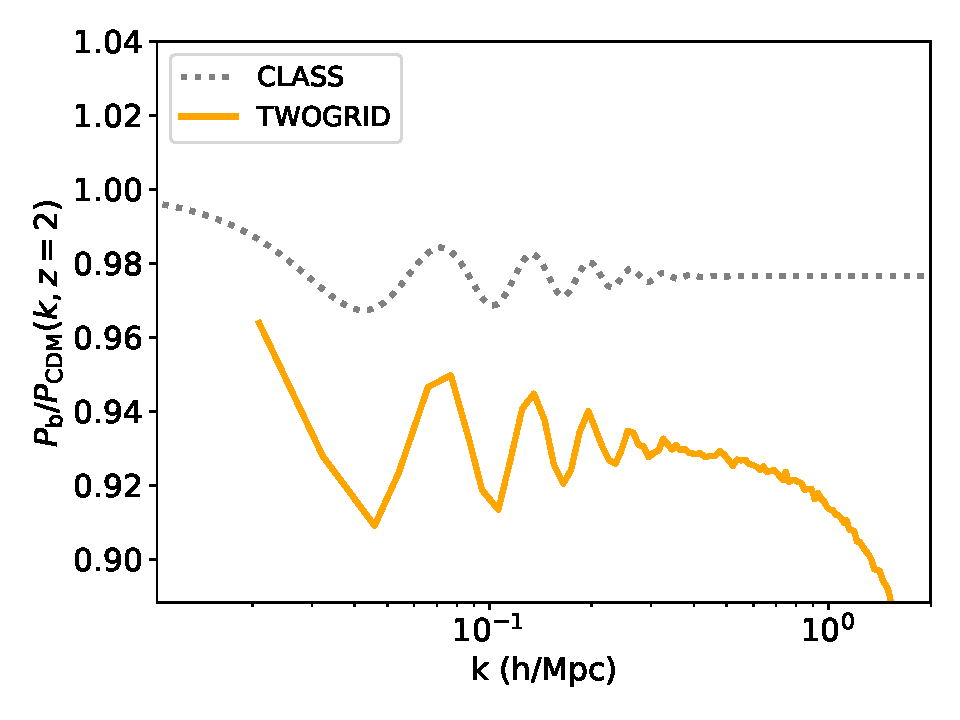
\includegraphics[width=0.5\textwidth]{plots/literature_2_relpower.pdf}
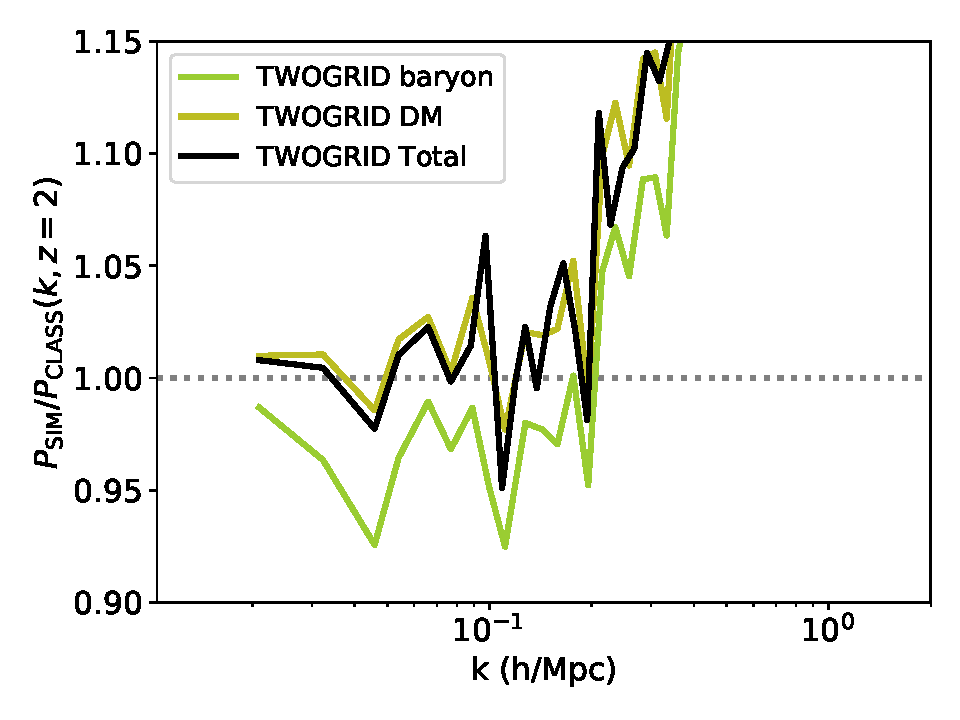
\includegraphics[width=0.5\textwidth]{plots/literature_2_class.pdf}
\caption{Results for the TWOGRID simulation, which initializes particles on two regular grids, offset by half a grid spacing. We have set $\sigma_8 = 0.008$ so that structure growth is linear even at late times. (Left) Ratio of baryon to CDM power spectra, $P_\mathrm{bar}/P_\mathrm{CDM}(k)$, at $z=2$ for the simulation (solid) and linear theory from CAMB (dash). (Right) Ratio of simulated to linear power spectra, $P_\mathrm{sim}/P_\mathrm{CLASS}(k)$ for gas (orange) and CDM (blue).}
  \label{fig:offsetgrids}
\end{figure}

\begin{figure}
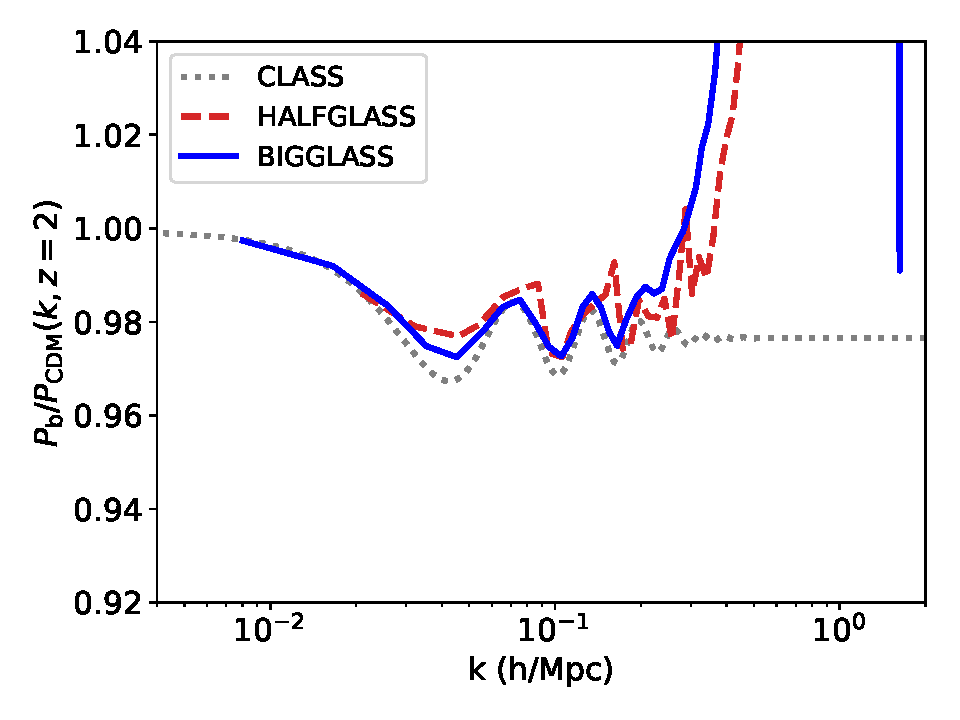
\includegraphics[width=0.5\textwidth]{plots/halfglass_2_relpower.pdf}
  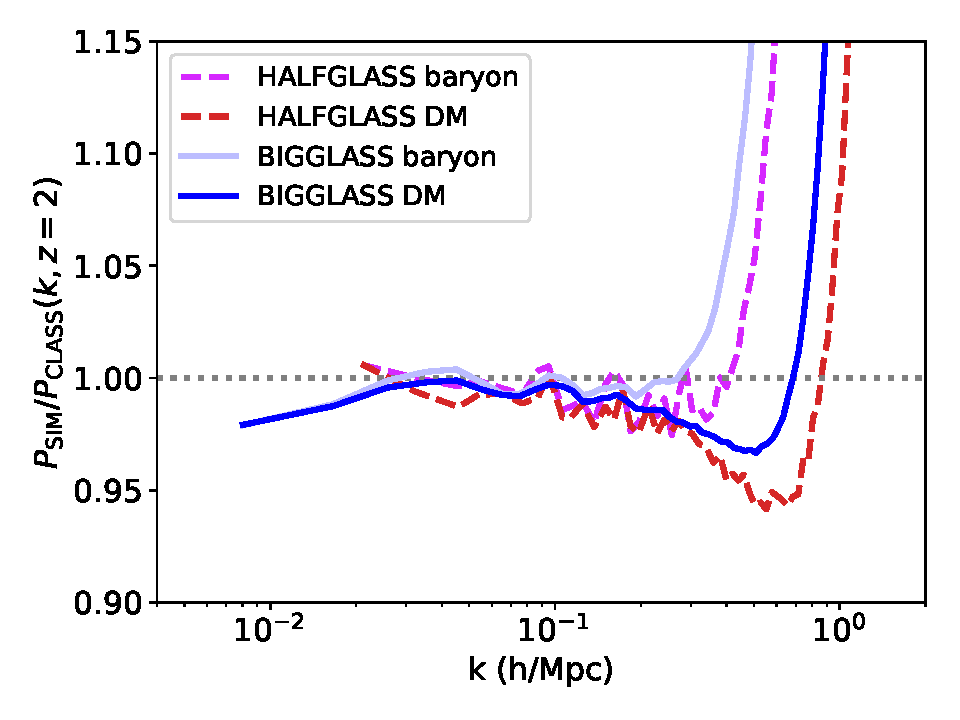
\includegraphics[width=0.5\textwidth]{plots/halfglass_2_class.pdf}
\caption{Results for our preferred simulation setup, where CDM is initialised with a regular grid and baryons are initialised with a glass. Shown are the HALFGLASS simulation, with $2\times 256^3$ particles in a $300$ Mpc/h box and the BIGGLASS simulation, with $2\times 768^3$ particles in a $1000$ Mpc/h box. We have set $\sigma_8 = 0.008$ so that structure growth is linear even at late times. (Left) Ratio of gas to CDM power spectra, $P_\mathrm{bar}/P_\mathrm{CDM}(k)$, at $z=2$ for the simulation (solid) and linear theory from CAMB (dash). (Right) Ratio of simulated to linear power spectra, $P_\mathrm{sim}/P_\mathrm{CLASS}(k)$ for gas (orange) and CDM (blue).}
  \label{fig:baryonglass}
\end{figure}

\begin{figure}
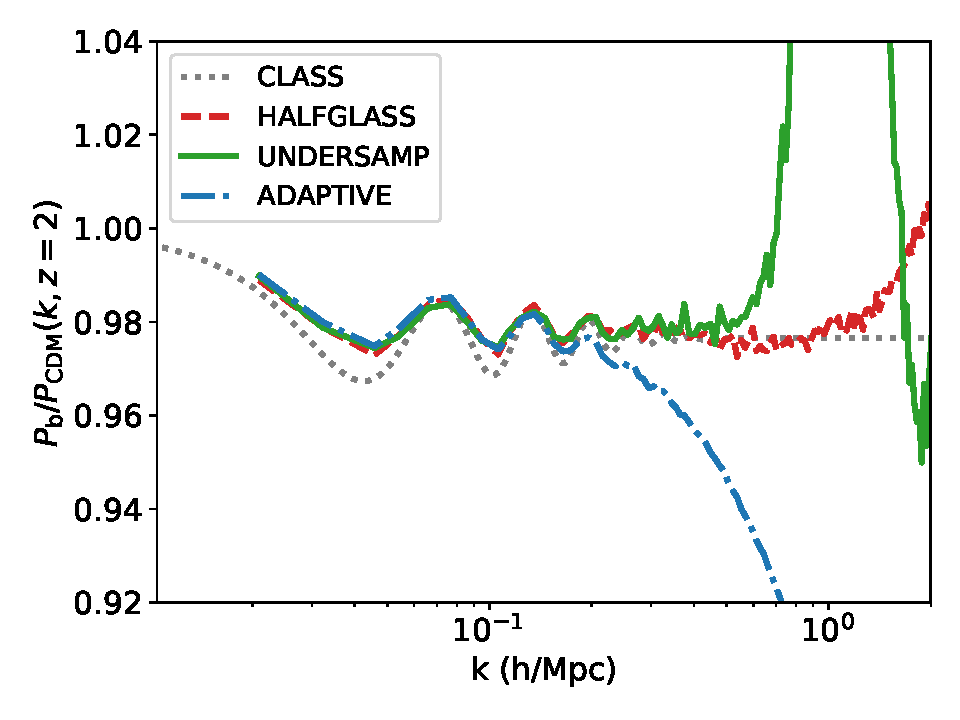
\includegraphics[width=0.5\textwidth]{plots/oversample_2_relpower.pdf}
  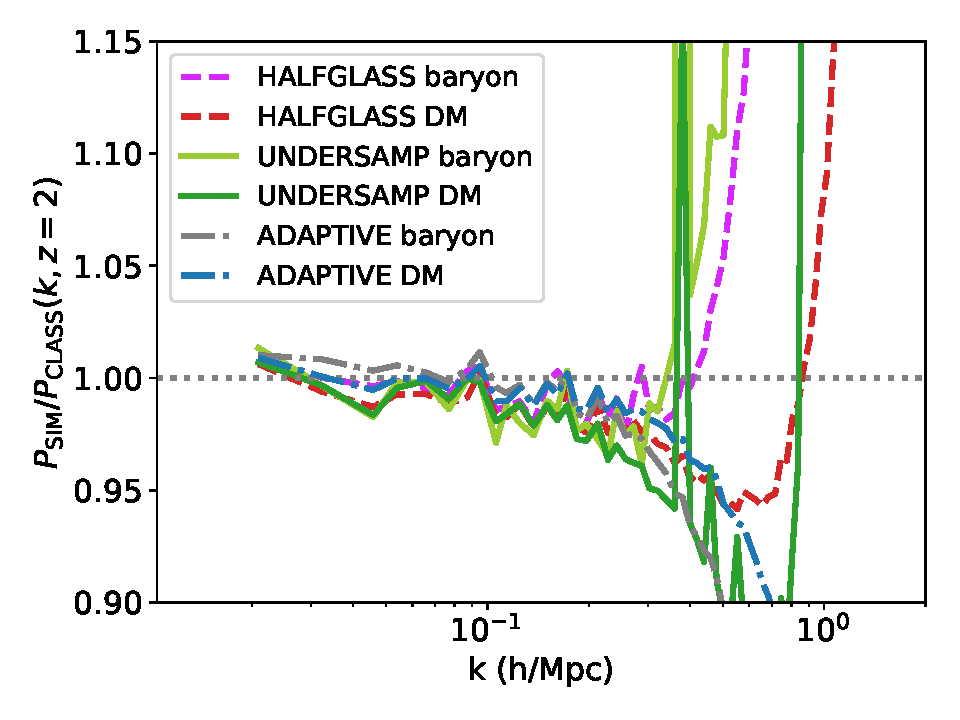
\includegraphics[width=0.5\textwidth]{plots/oversample_2_class.pdf}
\caption{Results for other simulation strategies successful at reproducing the relative power of baryons and CDM. Shown are: (ADAPTIVE) initializing particles on two regular grids, offset by half a grid spacing, but with particles evolved using an adaptive softening length for the gas. (UNDERSAMP) Using two regular grids with the number of CDM particle $5$ times larger than the number of baryon particles. Also show is the HALFGLASS simulation, for comparison. We have set $\sigma_8 = 0.008$ so that structure growth is linear even at late times. (Left) Ratio of gas to CDM power spectra, $P_\mathrm{bar}/P_\mathrm{CDM}(k)$, at $z=2$ for the simulation (solid) and linear theory from CAMB (dash). (Right) Ratio of simulated to linear power spectra, $P_\mathrm{sim}/P_\mathrm{CLASS}(k)$ for gas (orange) and CDM (blue).}
  \label{fig:adaptive}
\end{figure}

Figure~\ref{fig:offsetgrids} shows the baryon and cold dark matter power spectra for a cosmological simulation, compared to the output of CLASS at the same redshift. This simulation, TWOGRID, was initialized using the standard method of two grids of particles, one for baryons and one for cold dark matter, offset by a constant factor. Figure~\ref{fig:offsetgrids} illustrates the problem we aim to solve. Although the total matter power spectrum obeys the linear predictions, scattering between the baryon and DM particles causes the DM power spectrum to be over-predicted and the baryon power spectrum to be under-predicted, leading to an error in the relative power spectrum. 
\AFR{Do we really understand why the measured high-k power is below linear theory? I find it very suspicious.}
This problem has been discussed in, for example, Ref.~\cite{Angulo:2013}, although the magnitude of the error in our simulation does not match their results, presumably because of differences in the setting up of the regular grid.

We have confirmed that these results are independent of the force accuracy of the simulation and are not connected to adaptive timestepping or the length of the timesteps. For the former, we have performed small simulations where the short range force was evaluated using an $N^2$ pairwise gravity solver, simulations where the tree opening angle was changed and simulations where the split scale between the short and long-range forces was altered. Although the total power in the box in some cases changed (to the extent expected given the new force accuracy) on small scales, the power ratio between the baryons and cold dark matter did not.
We also confirmed that our results were the same when all particles had the same timestep and when the long-range PM timestep $4$ shorter. We have also confirmed that our results are independent of box size and particle number.

Figure~\ref{fig:baryonglass} shows the baryon and cold dark matter power spectra for cosmological simulations initialized using a glass for the baryons, generated using the procedure described in Section~\ref{sec:glass}. The agreement with linear theory is substantially improved, demonstrating that a Lagrangian glass can suppress the unphysical scattering between the baryonic and DM particles.

This result may at first appear puzzling. Effects of the particle grid should be confined to small scales close to the mean inter-particle separation. However, because the grid structure is repeated across the whole box, each baryonic particle encounters the same scattering force, and so the effect is also replicated across the box and shows up as a scale-independent error.

Using a Lagrangian glass for the baryons does not completely prevent unphysical force scatterings, but, because the particles are distributed irregularly, it ensures that the effect of this scattering is confined to small scales and does not change the large-scale growth. The glass does produce a noise power proportional to $k^4$ which in our case causes spurious small-scale growth. Since these are caused by the baryons, they would however be suppressed in a realistic simulation following gas pressures. Their relative importance would also be suppressed if we had not suppressed the initial power spectrum to ensure purely linear growth.
\AFR{How about running a simulation with hydro on? And may be with 10\% power instead of 1\%? I'm really worried about how bad the power is at k=0.5 h/Mpc. We argue that the noise would be lower with hydro, but I'm not sure how much to trust this without running an actual test.} 

As described in appendix B of Ref.~\cite{OLeary:2012}, the unphysical scatterings shown in Figure~\ref{fig:offsetgrids} occur because of the unequal particles masses, which allow dark matter particles to occasionally capture individual baryon particles. This motivates
an alternative solution to the relative power spectrum problem: changing the relative numbers of DM and baryon particles so that the per-particle mass is the same. For equivalent particle load this reduces the spatial resolution in the baryons by a factor of $\Omega_\mathrm{CDM}/\Omega_\mathrm{b} \sim 5$, which may not be desirable. However, it completely avoids the problem of unphysical particle captures and scatterings and, unlike the Lagrangian glass, does not introduce $k^4$ noise. Figure~\ref{fig:adaptive} shows the results of a simulation using this technique, confirming that it is also able to reproduce the baryon to DM power spectrum ratio on large scales at the cost of some Poisson noise in the power spectrum arising from poorer sampling.
\AFR{Chris showed that oversampling one of the species caused very strange power spectra at high-z, it looked quite suspicious. It would be great to add an appendix redoing the comparison at z=9 or so.}

Finally, we have checked that simulations which include adaptive gravitational softenings or disable the short-range tree force both reproduce the linear theory power spectra ratios on large scales, as suggested by Ref.~\cite{Angulo:2013}. Adaptive gravitational softenings avoid unphysical scatterings because the gravitational force is suppressed on scales less than that of the long-range particle mesh grid (in our simulations, 1/2 the mean interparticle spacing). Note that at high redshift, when the particle distribution is homogeneous, adaptive gravitational softenings are equivalent to disabling the short-range tree force.
Figure~\ref{fig:adaptive} shows the results, demonstrating that the loss of resolution is similar to undersampling the baryonic particles. Note that if a single particle is of sufficiently low mass to be Jeans stable, adaptive softenings are the physical thing to do \cite{Fire2:2018}. However, our simulations are of relatively low resolution and our particles are not near this threshold.

Compared to our preferred technique of using a Lagrangian glass for the baryonic particles, Figure~\ref{fig:adaptive} shows that both baryon undersampling and adaptive softenings produce similar results for the power spectrum. We prefer the use of Lagrangian glass because undersampling of baryons will negatively affect star formation models (which would be under-resolved), while using adaptive softenings leads to poor resolution in low-density areas, such as those which give rise to the Lyman-alpha forest.

\section{Conclusions}

We have shown that the spurious coupling present in N-body simulations between unequal mass CDM and baryon particles can be prevented from affecting the large scale power by setting the initial distribution of baryon particles with a Lagrangian glass. The CDM is initially placed on a grid. Chance juxtapositions of CDM and baryons are avoided by evolving the combined particle distribution with a reversed gravitational force, as in glass generation. This procedure allows a simulation to reproduce linear expectations for the power spectrum ratio between different particle species while avoiding the suppression of small scale power that results from increasing the gravitational softening length. We also explain an alternative possibility: over-sampling the CDM particles so that each particle species has the same mass, and demonstrate that this also reproduces linear expectations for the power spectrum ratio between different particle species.

\acknowledgments

We thank Matt McQuinn, Pat McDonald and Matias Zaldarriaga for helpful discussions. SB was supported by NSF grant AST-1817256. Computing resources were provided by NSF XSEDE allocation AST180058.
\AFR{I'd also like to thank Jose Onorbe and Paco Villaescusa-Navarro, we exchanged several emails about this. We also had several chats with Andrew Pontzen, Martin Rey and Tom Kitching, here at UCL.}


\bibliographystyle{JHEP}
\bibliography{offset}
\end{document}
